%%%%%%%%%%%%%%%%%%%%%%%%%%%%%%%%%%%%%%%%%
% Beamer Presentation
% LaTeX Template
% Version 1.0 (10/11/12)
%
% This template has been downloaded from:
% http://www.LaTeXTemplates.com
%
% License:

% CC BY-NC-SA 3.0 (http://creativecommons.org/licenses/by-nc-sa/3.0/)
%
%%%%%%%%%%%%%%%%%%%%%%%%%%%%%%%%%%%%%%%%%

%----------------------------------------------------------------------------------------
%	PACKAGES AND THEMES
%----------------------------------------------------------------------------------------

%\documentclass{beamer}

\documentclass[handout]{beamer}

\mode<presentation> {

% The Beamer class comes with a number of default slide themes
% which change the colors and layouts of slides. Below this is a list
% of all the themes, uncomment each in turn to see what they look like.

\usetheme{default}
%\usetheme{AnnArbor}
%\usetheme{Antibes}
%\usetheme{Bergen}
%\usetheme{Berkeley}
%\usetheme{Berlin}
%\usetheme{Boadilla}
%\usetheme{CambridgeUS}
%\usetheme{Copenhagen}
%\usetheme{Darmstadt}
%\usetheme{Dresden}
%\usetheme{Frankfurt}
%\usetheme{Goettingen}
%\usetheme{Hannover}
%\usetheme{Ilmenau}
%\usetheme{JuanLesPins}
%\usetheme{Luebeck}
\usetheme{Madrid}
%\usetheme{Malmoe}
%\usetheme{Marburg}
%\usetheme{Montpellier}
%\usetheme{PaloAlto}
%\usetheme{Pittsburgh}
%\usetheme{Rochester}
%\usetheme{Singapore}
%\usetheme{Szeged}
%\usetheme{Warsaw}

% As well as themes, the Beamer class has a number of color themes
% for any slide theme. Uncomment each of these in turn to see how it
% changes the colors of your current slide theme.

%\usecolortheme{albatross}
%\usecolortheme{beaver}
%\usecolortheme{beetle}
%\usecolortheme{crane}
%\usecolortheme{dolphin}
%\usecolortheme{dove}
%\usecolortheme{fly}
%\usecolortheme{lily}
%\usecolortheme{orchid}
%\usecolortheme{rose}
%\usecolortheme{seagull}
\usecolortheme{seahorse}
%\usecolortheme{whale}
%\usecolortheme{wolverine}

\setbeamertemplate{footline} % To remove the footer line in all slides uncomment this line
%\setbeamertemplate{footline}[page number] % To replace the footer line in all slides with a simple slide count uncomment this line

\makeatletter
\setbeamertemplate{footline}
{
  \leavevmode%
  \hbox{%
  \begin{beamercolorbox}[wd=.333333\paperwidth,ht=3.2ex,dp=1ex,center]{author in head/foot}%
    \usebeamerfont{author in head/foot}\insertsection
  \end{beamercolorbox}%
  \begin{beamercolorbox}[wd=.333333\paperwidth,ht=3.2ex,dp=1ex,center]{title in head/foot}%
    \usebeamerfont{title in head/foot}\insertsubsection
  \end{beamercolorbox}%
  \begin{beamercolorbox}[wd=.333333\paperwidth,ht=3.2ex,dp=1ex,right]{date in head/foot}%
    \usebeamerfont{date in head/foot}\insertauthor \,  Ph.D. defense \hspace*{2em}
    \insertframenumber{} / \inserttotalframenumber\hspace*{2ex} 
  \end{beamercolorbox}}%
  \vskip0pt%
}
\makeatother

%\setbeamertemplate{navigation symbols}{} % To remove the navigation symbols from the bottom of all slides uncomment this line
}
\addtobeamertemplate{navigation symbols}{}{%
    \usebeamerfont{footline}%
    \usebeamercolor[fg]{footline}%
    \hspace{1em}%
    \insertframenumber/\inserttotalframenumber
}

\newcommand*{\mathcolor}{}
\def\mathcolor#1#{\mathcoloraux{#1}}
\newcommand*{\mathcoloraux}[3]{%
  \protect\leavevmode
  \begingroup
    \color#1{#2}#3%
  \endgroup
}
\newcommand{\fc}{\mathfrak{c}}



\usepackage{macros}
\usepackage{color}
\usepackage{algpseudocode}
\usepackage{algorithmicx}
\usepackage{algorithm}
\usepackage{physics}
\renewcommand{\algorithmicrequire}{\textbf{Input:}}
\renewcommand{\algorithmicensure}{\textbf{Output:}}

%\usepackage{handoutWithNotes}
%\pgfpagesuselayout{3 on 1 with notes}[a4paper, border shrink=5mm]
\usepackage{tikz-cd}

%\usepackage{graphicx} % Allows including images
\usepackage{booktabs} % Allows the use of \toprule, \midrule and \bottomrule in tables
%----------------------------------------------------------------------------------------
%	TITLE PAGE
%----------------------------------------------------------------------------------------

\DeclareMathOperator{\cond}{cond}

\title[thesis defense]{Computational aspects of modular parametrizations \\ of elliptic curves} % The short title appears at the bottom of every slide, the full title is only on the title page

\author{Hao Chen} % Your name
\institute[UW] % Your institution as it will appear on the bottom of every slide, may be shorthand to save space
{
University of Washington Ph.D. defense \\ % Your institution for the title page
\medskip
Advisor: William Stein % Your email address
}
\date{April 26, 2016} % Date, can be changed to a custom date

\begin{document}

\begin{frame}
\titlepage % Print the title page as the first slide
\end{frame}


%
%\begin{frame}
%\frametitle{Overview} % Table of contents slide, comment this block out to remove it
%\huge \tableofcontents[hideallsubsections] % Throughout your presentation, if you choose to use \section{} and \subsection{} commands, these will automatically be printed on this slide as an overview of your presentation
%\end{frame}

%----------------------------------------------------------------------------------------
%	PRESENTATION SLIDES
%----------------------------------------------------------------------------------------

%\begin{frame}
%\tableofcontents
%\end{frame}

%------------------------------------------------
\section{Critical subgroups of elliptic curves} % Sections can be created in order to organize your presentation into discrete blocks, all sections and subsections are automatically printed in the table of contents as an overview of the talk
%------------------------------------------------

% A subsection can be created just before a set of slides with a common theme to further break down your presentation into chunks
 \begin{frame}
 \frametitle{\insertsection}
 \tableofcontents[currentsection]
 \end{frame}

%-------------
\subsection{Elliptic curves and modular curves}

\begin{frame}
\frametitle{Elliptic curves over $\bQ$}
\begin{Def}
An \red{elliptic curve} over $\bQ$ is a nonsingular projective curve $E \subseteq \bP^2$ with defining equation 
\begin{equation*}
y^2z = x^3 + Axz^2+Bz^3, 
\end{equation*}
where $A,B \in \bQ$ and  $4A^3+27B^2 \neq 0$.
\end{Def}

% The {\bf invariant differential}:  $\omega_E = \frac{dx}{y}$.

%$E(\bC)$ is a Riemann surface of genus 1, which is topologically a torus. % $E(\bQ)$ = The subgroup of rational solutions to \ref{eq:1}.

\pause

\begin{theorem}[Mordell-Weil]
$E(\bQ)$ is a finitely generated abelian group, i.e., $$E(\bQ) \cong \bZ^r \oplus T,$$
for some $r \geq 0$ and $T$ finite. 
\end{theorem}
$r$ is called the \red{rank}. $T$ is the \red{torsion subgroup}. 

\end{frame}

%\begin{frame}
%\frametitle{Group law on elliptic curves(I)}
%\centering
%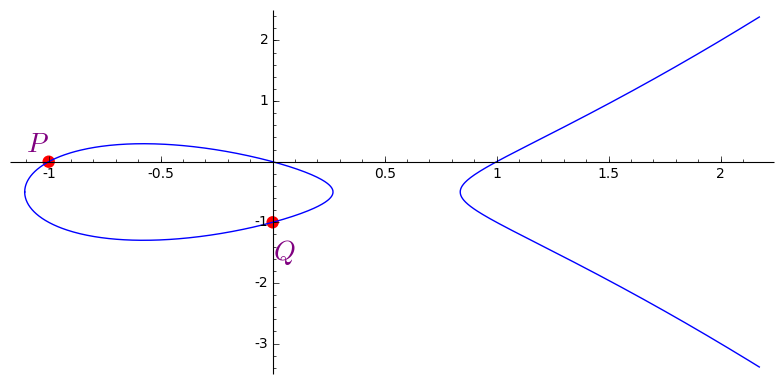
\includegraphics[width=0.8\linewidth]{pics/1.png}
%\end{frame}

%\begin{frame}
%\frametitle{Group law on elliptic curves(II)}
%\centering
%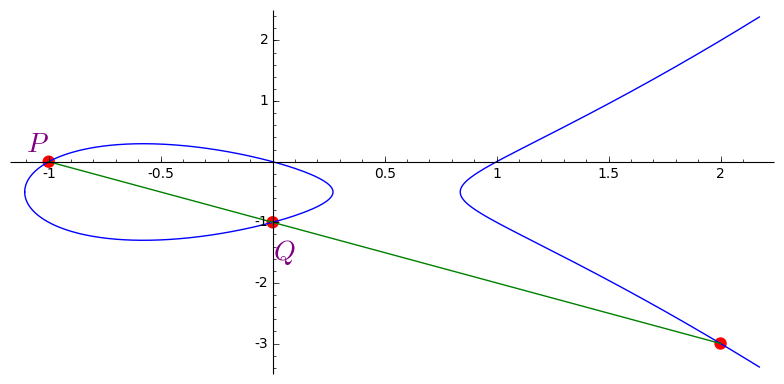
\includegraphics[width=0.8\linewidth]{pics/2.png}
%\end{frame}

\begin{frame}
\frametitle{The BSD conjecture} 


% $rank(E(\bQ))$ has been studied extensively in number theory. \\ % up to now, no easy way of computing the rank.
There is an entire function $L(E,s)$ called the $L$-function of $E$.  \\

\medskip
\pause

The rank part of the  \red{Birch and Swinnerton-Dyer (BSD) conjecture} is:
\begin{equation*}
	rank(E(\bQ)) = \ord_{s=1}L(E,s).
\end{equation*}

\pause
\medskip

\begin{itemize}
\item $\ord_{s=1}L(E,s)$ is the \red{analytic rank}, denoted by \red{$r_{an}(E)$}. \\
\item The BSD conjecture is open when $r_{an}(E) > 1$. \\
\item The proof of rank BSD for $r_{an}(E) \leq 1$ uses Heegner points. 
\end{itemize}

\end{frame}


%------------------------------------------------

\begin{frame}
\frametitle{Modular curves}
Let $N \geq 1$ be an integer, consider the group 
\[
	\Gamma_0(N) = \left \{ \abcd{a}{b}{c}{d} \in SL_2(\bZ): N \mid c \right\}.
\]
$\cH^* := \{z \in \bC: im(z) > 0\} \cup \bP^1(\bQ)$.  $\Gamma_0(N)$ acts on $\cH^{*}$. 

\begin{Def}
$X_0(N) = \Gamma_0(N) \backslash \cH^*$ is the modular curve of level $N$. 
\end{Def}

\begin{itemize}
\item $X_0(N)$ is a  nonsingular projective curve.
\item Rational functions on $X_0(N)$ have \red{$q$-expansions} at infinity:
\[
	u(q)  = \sum_{n \geq -m} b_n q^n, \; q = e^{2 \pi i z}. 
\]
\end{itemize}
\end{frame}

\begin{frame}
\frametitle{The modularity theorem}
%Notation: for a cusp form f weight 2 and level $N$, let $\omega = f(z)dz$.

%\begin{Fact}
%$\omega$ is a holomorphic differential on $X_0(N)$.
%\end{Fact}

\begin{theorem}[Modularity]
For every elliptic curve $E/\bQ$, there exists an integer $N > 1$ and a surjective morphism 
$\varphi: X_0(N) \to E$ defined over $\bQ$.
\end{theorem}

\pause
\smallskip

The smallest $N$ is called the conductor of $E$.  \\
\smallskip

Let $\omega = \varphi^*(\frac{dx}{y})$. Then $\omega = c f(z) \mathrm{d} z$, where $f$ is the \red{modular form attached 
to $E$}.  \\

\smallskip

We assume $E$ is optimal. Then $\varphi$ is unique up to sign.


Idea:  use $\varphi$ to find points on $E$ from special points on $X_0(N)$. 

-- rational points on $X_0(N)$ -- cusps. 
-- Heegner points. 
-- Ramification points. 
-- Others?? 

Note: up to now, no known construction in $\geq 2$. 


\end{frame}

% Note: the elliptic points, when they exist, are Heegner points on $X_0(N)$.

% nothing to do with level.
%From the Gross-Zagier formula, we can derive:

\subsection{The critical subgroup and critical polynomials}

\begin{frame}{The critical subgroup $E_{crit}(\bQ)$}
%\frametitle{Background: Ramification}

%Given any morphism $\varphi: X \to Y$ between curves, the ramification divisor of $\varphi$ is 
%\[
%	R_\varphi = \sum_{x \in X} (e_\varphi(x) - 1) [x]
%\]
%there is a finite set of points $x \in X$ where 
%the preimage $\varphi^{-1}(\varphi(x))$ is `smaller than usual'. Such x is called a {\bf critical point}, 
%and $f(x)$ is called a ramification point. 
%For example, the projection $\{(x,y) \in \bR^2: x = y^2\} \to \bR: (x,y) \mapsto x$ 
%is ramified at $(0,0)$.

%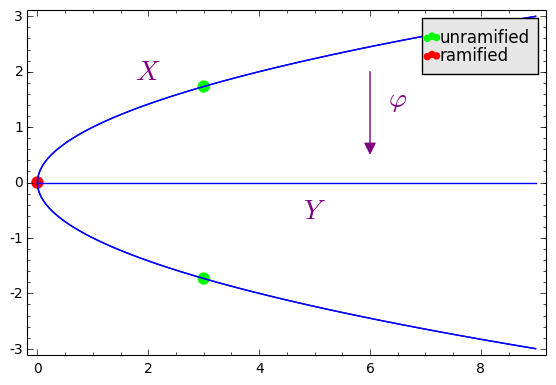
\includegraphics[width=10cm,height=7cm]{pics/ramification.png}


%\end{frame}

%\begin{frame}{Riemann-Hurwitz Formula}
%Some of on divisors: 
%\begin{itemize}
%\item A {\bf divisor} $D$ on a curve $X$ is a finite formal sum of points $D = \sum_{x \in X} n_x[x]$, $n_x \in \bZ$.\\
%\item $\supp D = \{x: n_x \neq 0\}$ = the {\bf support} of the divisor. 
%\item For $f \in \bQ(X)$, $\Div(f) = \{\mbox{zeros of } f\} - \{\mbox{poles of } f\}$.
%\item Divisor of differentials are defined similarly. 
%\end{itemize}

%For every $\varphi: X \to Y$, there exists a divisor $R_{\varphi} \geq 0$, called 
%the \textbf{ramification divisor} of $\varphi$, such that 
%$\supp R_{\varphi} = \mbox{ critical points of } \varphi$.

%\begin{theorem}[Riemann-Hurwitz formula]
%If $\varphi: X \to Y$ is a non-constant morphism of curves and $\omega$ is any differential on $X$, then 
%\[
%          \Div(\varphi^*(\omega))   = \varphi^*(\Div(\omega)) + R_{\varphi}.
%\]
%\end{theorem}
% Let $\varphi: X_0(N) \to E$ be the modular parametrisation and let 


Let $R_\varphi$ be the ramification divisor.

\begin{Def}[Mazur, Swinnerton-Dyer]
The \red{critical subgroup} of $E$ is
\[
	E_{crit}(\bQ)  = \langle tr(\varphi([z])) : [z] \in \supp R_\varphi \rangle \subseteq E(\bQ), 
\] 
where $tr(P) = \sum_{\sigma: \bQ(P) \to \bar{\bQ}} P^{\sigma}$.
\end{Def}

\pause



\begin{itemize} 
%\item $R_\varphi$ is a rational divisor. Therefore, for any $e\in \supp R_\varphi$, we have $\varphi(e) \in E(\bar{\bQ})$.
%\item C.Delaunay described an algorithm to compute $R_\varphi$ using a complex analytic method.
\item $R_\varphi = \Div(\omega)$. In particular, $\deg R_{\varphi} = 2g(X_0(N))-2$. \\
\end{itemize}
%Riemann-Hurwitz formula + $\Div(\omega_E) = 0$  $\implies .
%(a canonical divisor on $X_0(N)$). \\

%$\varphi$ is ramified at $2g-2$ points, counting  multiplicity.
%  F.Brunault: a sufficient condition such that $R_\varphi$ 
%does not contain cusps

\begin{question}[Mazur and Swinnerton-Dyer, 1974]
Is there an elliptic curve $E/\bQ$ with $r_{an}(E) \geq 2$ and $rank(E_{crit}(\bQ)) >0$?
\end{question}

 % Then he uses a complex form of modular parametrisation to compute $E_{crit}(\bQ)$.

\end{frame}

%------------------------------------------------





\begin{frame}{Critical $j$-polynomial}
%The group $E(\bQ)$ has been studied extensively in number theory.
%Associated to $E$ is an analytic function $L(E,s)$( the L-function of E). \\
%The rank part of the B-SD conjecture states
%\[
%	rank(E(\bQ)) = \ord_{s=1}L(E,s).
%\] 
%It is proved for $\ord_{s=1}L(E,s) \leq 1$.


%\end{frame}

%\subsection{Critical Polynomial}
%\begin{frame}
%\frametitle{Critical Polynomials}

%Notation: $Z_\omega =$.  \\

To help compute $E_{crit}(\bQ)$, we make the following definition. 
\begin{Def}
%Let $E/\bQ$ be an elliptic curve of conductor $N$ and let $j$ be the $j$-invariant. 
Write $\Div(\omega) = \sum n_z[z]$. The \red{critical j-polynomial} of $E$ is 
\[
F_{E,j}(x) = \prod_{z \in \supp \Div(\omega), j(z) \neq \infty}(x-j(z))^{n_z}.
\]
\end{Def}
$F_{E,j}(x) \in \bQ[x]$ and $\deg F_{E,j} \leq 2g-2$ (equality holds if $N$ is square free). 

\pause
\medskip

For $h \in \bQ(X_0(N))$, can define $F_{E,h}(x)$. 


\end{frame}

%------------------------------------------------

\begin{frame}{Polynomial Relation (I)}
%When  $N$ is not square free, \textbf{NORM} does not work. \textbf{IPR} is an algorithm to compute $F_{E,j}$, which works for any $N$. \\
Let
\[
r := j(j-1728)  \frac{\omega }{{d j}}, \;  u := \frac{1}{j}.
\]
Then $r, u \in \bQ(X_0(N))$, and $\Div_0(r)  = \Div(\omega) + D_0$, where points in $\supp D_0$ have $j$-value 0 or 1728.  \\

\smallskip 

\pause

%Moreover, if $T >  2g-2$, then the pair $(rj^T,u)$ satisfies the conditions of the proposition. (\hyperlink{condition is satisfied}{\underline{One proves it by looking at the zeros and poles of $rj^T$}}). % Proof is not long, but please believe me. t

\begin{Prop}[C.]
For $T \gg 0$, let $P(x,y) = f_n(y)x^n + \cdots + f_1(y)x + f_0(y)$ be an irreducible polynomial over $\bZ$ such that 
$P(rj^T, u) = 0$. Then
\[
		F_{E,j}(x) = f_0(1/x) \cdot x^{A} (x - 1728)^B
\]	
where $A,B$ are explicitly computable. 
\end{Prop}

\end{frame}

\begin{frame}{The Algorithm}

\begin{algorithm}[H]
\begin{algorithmic}[[1]
\Require The newform $f_E$ attached to elliptic curve $E/\bQ$; 
\Ensure $F_{E,j}$.  
\smallskip
\State $r = \frac{j(j-1728) f_E  dz }{dj}, \;  u = \frac{1}{j}$. 
\State Compute the q-expansions of $r$ and $u$ to precision $q^M$. 
\State Solve the linear equations $\sum c_{a,b}r(q)^au(q)^b = 0 \pmod {q^M} $ for $c_{a,b}$. 
\State Set $P(x,y) = \sum c_{a,b}x^ay^b$ and apply the proposition. 
\end{algorithmic}
\end{algorithm}

Let $H_d$ be the Hilbert class polynomial of disc $d$. 
\begin{Example}
$F_{{\bf 44a},j}(x) = H_{-44}(x)^2$. $F_{{\bf 37a},j}(x) = H_{-148}(x)$. $F_{{\bf 37b},j}(x) = H_{-16}(x)^2$.
\end{Example}

%Remark: When $N$ is large($\sim 1000$), the algorithm {\bf PR} is slow. We have 
%\hyperlink{yang pair}{\underline{another faster algorithm}} that computes a critical $h$-polynomial, where $h$ is some $\eta$-quotient chosen within the algorithm.

\end{frame}


%\begin{frame}{More examples of critical $j$-polynomials computed via the {\bf IPR} algorithm}
%\begin{Example}
%$E = \textbf{197a}$, we obtain
%\[
%	F_{E,j}(x)  = (x + 884736)^2 H_{-197 \cdot 4}(x) f_{18}(x),
%\]
%where $f_{18}$ is an irreducible polynomial in $\bQ[x]$ of degree 18.
%\end{Example}

%\begin{Example}
%\label{ex: 389a}
%$E = \textbf{389a}$, the curve of algebraic rank 2 with smallest conductor. 
%\[
%	F_{E,j}(x)  = (x + 884736)^2 f_{60}, 
%\]
%where $f_{60}$ is irreducible of degree 60. 
%This example will be revisited in Section ~\ref{sec:exact points}. 
%\end{Example}

%\pause



% \hyperlink{yang pair}{Yang pair}


%\end{frame}

%------------------------------------------------

%\begin{frame}{Integer Polynomial Relation(IPR): Example}
%\begin{Example}
%$E = \textbf{44a}$,
%\begin{align*}
%F_{E,j}(x) &= (x^{3} - 1122662608x^{2} + 270413882112x - 653249011576832)^2  \\
%            &= H_{-44}(x)^2.
%\end{align*}
%\end{Example}

%\begin{Example}
%$E = \textbf{48a}$, $F_{E,j}(x) = 1$. Explanation: All critical points are cusps. In fact, $Z_{\omega}  = [1/4] + [3/4] + [1/12] +[7/12]$. 
%\end{Example}


%\end{frame}


%------------------------------------------------
%\section{Algorithm: Yang pair}

%\begin{figure}
%\includegraphics[width=0.8\linewidth]{test}
%\end{figure}


%------------------------------------------------

%Remark: once we have $F(r_1, h_2) = 0$, let $F_0(x) = F(0,h_2)$. Then $F_{E,h} =  F(0,h_2)/(*)$, where $(*)$ the extra factor  coming from zeros of $h_1$. $(*)$ is explicitly computable, but we may also `eyeball' it. \\




%------------------------------------------------
\subsection{Computing the critical subgroup}

\begin{frame}{The critical subgroup $E_{crit}(\bQ)$}

% Recall the definition: $E_{crit}(\bQ) = \langle tr(\varphi(e)): e \in \supp \Div(\omega)\rangle$. We observe that 

%Write $Z_\omega = \sum_{i = 1}^n n_i S_i$, where the $n_i \in \bZ_{\geq 1}$ and each $S_i$ is a sum of points in a Galois orbit. Set $P_i = \sum \varphi_*(S_i) \in E(\bQ)$. Let $E_{crit}^u(\bQ)  = \langle \{P_i\}_i \rangle$.
%\begin{Lemma}
%$E_{crit}(\bQ) \otimes \bQ = E_{crit}^u(\bQ) \otimes \bQ$, i.e., $E_{crit}^u(\bQ)$ and  $E_{crit}(\bQ)$ have the same rank as abelian groups.
%\end{Lemma}


%\begin{itemize}
%\item Observation: $g = \frac{f\Delta}{E_4^2E_6} \in \bQ(X_0(N))$.  \\
%\item Therefore, $\varphi_*(\Div(g)) = \Div(\varphi_*(g))$(i.e., it is a principal divisor). \\
%\item However, if $D = \sum n_P[P]$ is a principal divisor on $E$, then $\sum n_P P = 0 \in E(\bQ)$. \\
%\item This gives a linear relation on the images of zeros of these four modular forms. 
%\end{itemize}
%\begin{align*}
%& \implies \varphi_*(\Div(g)) = 0 \in Div^0(E) \\
%& \implies \sum_{z \in \Div(g)} n_z\varphi(z) = 0 \in E(\bQ). 
%\end{align*}

%Recall the lemma: 
%\begin{Lemma}[C.]
%$6 P_{all} =  - 3 \sum_{c \in Ell_2(N)} \varphi(c) - 4 \sum_{d \in Ell_3(N)} \varphi(d)$. \\
%\end{Lemma}

% If $r_{an}(E) \geq 2$, then the right hand side is torsion by Gross-Zagier, hence

%\begin{Prop}[C.]
%Assume either $r_{an}(E) \geq 2$ or $X_0(N)$ has no elliptic point. Then $P_{all} \in E(\bQ)_{tors}$,  hence $rank(E_{crit}(\bQ)) \leq n_{\omega} - 1$. 
%\end{Prop}
%\pause

%If in addition $r_{an}(E)$ is even, then $w_N(\varphi(e)) \equiv - \varphi(e) \pmod {E(\bar{\bQ)}_{tors}}$ for all $e \in X_0(N)$.
\begin{Theorem}[C.]
\label{cor: cm}
%Let $E/\bQ$ be an elliptic curve of conductor $N$. 
Suppose $r_{an}(E) \geq 2$, and assume at least one of the following holds: \\
(1) $F_{E,j} = \prod_{m =1}^k H_{D_m}^{s_i}\cdot F_0$, where 
$\bQ(\sqrt{D_m}) \neq \bQ(\sqrt{D_n})$ for all $m\neq n$, and $F_0$ is irreducible. \\
(2) $F_{E,h}$ is irreducible for some non-constant function $h \in \bQ(X_0(N))$. \\
Then $rank(E_{crit}(\bQ))  = 0$. 
\end{Theorem}
\end{frame}


%------------------------------------------------

\begin{frame}
\frametitle{Critical polynomials for elliptic curves of rank 2 and conductor $<1000$ (I)}
\begin{center}
   \begin{table}[h!]
    \begin{tabular}{ | l | l | l | |p{4.4cm}  |}
    \hline
    $E$ & $g(X_0(N))$    & $h$ & $\mbox{ Factorization of } F_{E,h}(x)$     \\ \hline \hline
    389a & 32  & $j$ & $H_{-19}(x)^2 (x^{60}+ \cdots)$ \\ \hline
    433a & 35  & $j$ &  $x^{68}+\cdots$  \\ \hline
     446d & 55  & $j$ &  $x^{108}+\cdots$ \\ \hline
    563a & 47  & $j$ &  $H_{-43}(x)^2 (x^{90} - \cdots)$   \\ \hline
    571b& 47  & $j$ &  $H_{-67}(x)^2 (x^{90} - \cdots)$ \\ \hline
    643a& 53  & $j$ &  $H_{-19}(x)^2 (x^{102} - \cdots)$ \\ \hline
    664a & 81    &   $\frac{\eta_4\eta_8^2 \eta_{332}^5}{\eta_{166}\eta_{664}^{6}{\eta_2}}$ & $x^{160} - \cdots$ \\ \hline
    655a& 65  & $j$ &  $x^{128} - \cdots$ \\  \hline
    681c& 75  & $j$ &  $x^{148} - \cdots$ \\  \hline
    707a & 67  & $j$ & $x^{132} - \cdots$ 
        \end{tabular}
    \label{table: rank two}	
   \end{table}
\end{center}


\end{frame}
 

\begin{frame}
\frametitle{Critical polynomials for elliptic curves of rank 2 and conductor $<1000$ (II)}   \begin{table}[h!]
    \begin{tabular}{ | l | l | l |p{4.4cm} |}
    \hline
    $E$ & $g(X_0(N))$    & $h$ & $\mbox{ Factorization of } F_{E,h}(x)$     \\ \hline \hline
    709a& 58  & $j$ &  $x^{114} - \cdots$\\ \hline
    718b& 89  & $j$ &  $ H_{-52}(x)^2 (x^{172} - \cdots)$\\ \hline
    794a& 98  & $j$ &  $H_{-4}(x)^2 (x^{192} - \cdots)$\\ \hline
    817a& 71  & $j$ &  $x^{140} - \cdots$\\ \hline
    
    916c & 113   & $j$ &$H_{-12}(x)^8(x^{216}+\cdots)$  \\ \hline
    
   % 916c & 113   & $\frac{\eta_2^7  \eta_{458}^5}{\eta_{229}\eta_{916}^6\eta_4^2 \eta_1^3}$ &\footnotemark $(x^2 - 28x + 3664)^2(x^2 + 116x + 3664)^2(x^{216}+\cdots)$  \\ \hline
    
    944e & 115    & $\frac{\eta_{16}^4 \eta_{4}^2}{\eta_8^6}$ & $x^{224} - \cdots$.\footnotemark \\ \hline 
    997b& 82  & $j$ &  $H_{-27}(x)^2 (x^{160} - \cdots)$\\ \hline
    997c& 82  & $j$ &  $x^{162} - \cdots$\\ \hline
    \end{tabular}
    \label{table: rank two}	
   \end{table}
   	\footnotetext[1]{Here 4 of the critical points are cusps, so $\deg F = 2g- 6$.}

\end{frame}

%------------------------------------------------


%All critical $j$-polynomials in the table are of the form $F_{E,j} = f_{CM}f_0$, so $E_{crit}(\bQ)$ is torsion in these cases. \\
%The critical $h$-polynomial for the curves \textbf{664a} and \textbf{994e} are irreducible, hence $E_{crit}(\bQ)$ is torsion for these two curves. \\ 
%The critical $h$-polynomial for the curve \textbf{916c} is not irreducible, but...\\
%the two quadratic factors in its factorisation correspond to CM points on $X_0(N)$ with j-value 54000. Therefore, $E_{crit}(\bQ)$ is torsion as well.  \\

\begin{frame}{Discussion}

\begin{Corollary}
For all elliptic curves $E$ of rank 2 and conductor $N <1000$, the rank of $E_{crit}(\bQ)$ is 0.
\end{Corollary}
\pause
\smallskip
Future work: 
\begin{itemize}
\item Compute $E_{crit}(\bQ)$ for $E = {\bf 5077a}$. 

Current method will take roughly  5500/(number of cpus) hours.  

\item Prove or disprove that $\rank(E_{crit}(\bQ)) = 0$ whenever $r_{an}(E)$ is even.

(For infinitely many?) 

\end{itemize}

\end{frame}



% Extra slides that I may not need.
%----------------------------------------------------------------------------------------



% modular forms
%----------------------------------------------------------------------------------------

\section{$q$-expansion of newforms at non-unitary cusps} 

 \begin{frame}
 \frametitle{\insertsection}
 \tableofcontents[currentsection]
 \end{frame}


\subsection{Problem description}



\begin{frame}
\frametitle{Modular forms}
Let $f$ be a function $f: \cH \to \bC$,  $\alpha  = \abcd{a}{b}{c}{d} \in SL_2(\bZ)$, and let $k \in \bZ$. The weight-k action of $\alpha$ on $f$ is
defined by
\[
	f|[\alpha]_k(z) := (cz+d)^{-k}f(\alpha z).
\]

\pause

\begin{Def}
A \textbf{modular form} of weight $k$ and level $N$ is a holomorphic function $f: \cH \to \bC$ s.t. \\
(1) $f(z)  = f|[\alpha]_k(z), \; \forall \alpha \in \Gamma_0(N)$ ($\Gamma_1(N)$). \\
(2) $f$ has holomorphic extension to all cusps of $X_0(N)$ ($X_1(N)$). \\
\end{Def}

\pause

\red{Cusp forms} = modular forms that are zero at all cusps. \\
Modular forms have \red{$q$-expansions}: $f(q) = \sum_{n \geq 0} a_n q^n$, $q = exp(2\pi i z)$. \\
The space of cusp forms = $S_k(N)$. 

\end{frame}


\begin{frame}{Operators on modular forms}

\begin{itemize}
\item Hecke operators: a family $\{T_n, n \geq 1 \} \cup \{ \langle d \rangle: (d,N) = 1\}$ of commuting linear operators on $S_k(N)$. 

\item $B_d$ and $U_d$ operators: $B_d(\sum a_n q^n) = \sum a_{n} q^{nd}$, $U_d(\sum a_n q^n) = \sum a_{nd} q^{n}$.

\item The Atkin-Lehner involution $W_N$.  If $f$ is a newform on $\Gamma_1(N)$, then 
\[
	f | W_N = w(f) \bar{f}
\]
$w(f) \in \bC_1$ is called the \red{pseudo-eigenvalue} of $f$. 

\end{itemize}

\end{frame}

\begin{frame}{Newforms}

\begin{itemize}
\item When $M \mid N$, $\exists$ degeneracy maps $S_k(M) \to S_k(N)$. 
\item Old subspace = span of images of all degenaracy maps. 
\item New subspace = $(\mbox{Old subspace})^{\perp}$.
\item $S_k(N)^{new}$ has a basis of simultaneous eigenforms for \red{all}  Hecke operators. These eigenforms 
are called \red{newforms}.
\end{itemize}

\end{frame}



\begin{frame}{Fourier expansion}
Let $f \in S_k(\Gamma_0(N))$ be a newform and let $\fc \in X_0(N)$ be a cusp other than $\infty$.  \\

Goal: compute the expansion of $f$ at $\fc$. \\ 

First, only well-defined for $denom(\fc)^2 \mid N$. \\ 

Equivalent to computing the expansion of 

$$\large{f | \left[\mtwo{1}{0}{\ell d}{1}\right]}$$ 
$\red{\mbox{ at } \infty} \mbox{ for all } d^2 \mid N$ and $\ell \in (\bZ/N\bZ)^{\times}$.

\end{frame}

\subsection{Deriving the formula}

\begin{frame}{Idea of computing}

Let $S_c' = \abcd{1}{\frac{1}{c'}}{0}{1}$ and $A_c' = \abcd{1}{0}{c'}{1}$.  Then 
\[
	A_c^{-u} = W_N S_{c'}^u W_N, \, \forall u \in \bZ. 
\]
For a character $\chi$ modulo $c'$, put 
\begin{equation*}
\label{formula: RS}
	f | \red{R_\chi(c')} := \sum_{u =0}^{c'-1} \bar{\chi}(u) f | S_{c'}^u.
\end{equation*}
$f|R_\chi(\cond \chi) = g(\bar{\chi})f_\chi$. ($f_\chi (q) = \sum a_n(f) \chi(n)  q^n$ is a modular form of level $N'$.)   We have \begin{equation} 
\label{formula}
	\varphi(c') A_c^{-a} = \sum_{\cond(\chi) \mid c'} \chi(a) W_N R_\chi(c') W_N. 
\end{equation}

Applying to $f$, we arrive at
\begin{equation} \label{expansion0}
	\boxed{f_{[\frac{a}{c}]} \left( q\right) = \frac{w(f) }{\varphi(c')}\sum_{\cond(\chi) \mid c'} \chi(-a) f| R_\chi(c')  W_N}
\end{equation}
\end{frame}


\begin{frame}{Idea (ctnd)}

Just need to compute $f| R_\chi(c') W_N$.  \\

Recall: $f \otimes \chi$ :=  the unique newform such that $a_p(f \otimes \chi) = a_p(f_\chi)$ for almost all $p$. 
(We call $f \otimes \chi$ the \red{twist of $f$ by $\chi$}). \\

\pause 
\medskip


When $c' = \cond(\chi)$ and $f_\chi = f \otimes \chi$, then  $f| R_\chi(c') W_N = w(f \otimes \chi) f_\chi$. 
\medskip

Otherwise, $f_\chi = (f \otimes \chi) | ( 1 - U_d | B_d)$, and we use 
\begin{Lemma}
   $$f| B_d|W_N = \left(\frac{N}{Md^2} \right)^{k/2}  w(f)  (f|B_{\frac{N}{Md}})^{*}.$$
\end{Lemma} 

\medskip

Conclusion: suffices to compute $f \otimes \chi$ and $w(f \otimes \chi)$.

\end{frame}

\subsection{Computing twists and pseudo-eigenvalues}

\begin{frame}{Algorithm for twists}

\begin{Lemma}
Let $\epsilon$ be the character of $f$. Then the level of $f \otimes \chi$ divides $lcm(N, \cond(\epsilon) \cond(\chi), \cond(\chi)^2)$. 
\end{Lemma}

\begin{Lemma}
For every $N \geq 1$, there exists an integer $B = B(N)$ such that if $g_1$, $g_2$ be two normalised newforms of levels $N_1,N_2$ dividing $N$ and 
\[
	a_n(g_1) = a_n(g_2), \, \mbox{for all }1 \leq n \leq B \mbox{ such that } \gcd(n,N) = 1,
\]
then $g_1 = g_2$.
\end{Lemma}

\end{frame}

\begin{frame}{Algorithm to compute $f \otimes \chi$}
\begin{algorithm}[H]
\caption{Identifying  $f \otimes \chi$}
\label{alg: twist}
\begin{algorithmic}
    \Require $f \in S_k(\Gamma_0(N))$ a normalized newform; 
     $\chi$ -- Dirichlet character of prime power conductor $Q = q^\beta$ ($Q^2 \mid N$). 
    \Ensure The newform $f \otimes \chi$. 
    \For{each $M \mid N$} 
	\State Compute a basis $\{g_1, \ldots, g_s\}$ of $S_k(M, \chi^2)^{new}$. 
    	\State $B$ := the Sturm bound for $\Gamma_1(MQ^2)$. 
    	\For{$1 \leq j \leq s$} 
		\If{$a_n(g_i)= a_n(f)\chi(n)$ for all $1 \leq n \leq B, \gcd(n,q) = 1$}
			\State \Return $g_i$.
		\EndIf
	\EndFor
   \EndFor
   \State \Return Error.
\end{algorithmic}
\end{algorithm}
\end{frame}

\begin{frame}{Computing the pseudo-eigenvalue}
Recall that modular symbols are linear combinations of $\{\alpha, \beta\}$, $\alpha, \beta \in \bQ \cup \infty$, 
and we put 
\[
	\langle f, \{\alpha, \beta\} \rangle := \int_{\alpha}^{\beta} f \textrm{d} z. 
\]
\begin{Lemma}[C.]
There exists a weight-$k$ modular symbol $M$ be such that $W_N(M) = N^{k/2 -1} M^*$. Moreover, if $\langle f, M \rangle \neq 0$, then 
\[
	w(f) = \frac{\langle f,M \rangle }{\overline{\langle f,M \rangle}}.
\]
\end{Lemma} 

\end{frame}

\begin{frame}{Examples (I)}

\begin{Example}
$E = {\bf 50a}$. $f_E$ is twist-minimal. Let  $\fc = [\frac{1}{10}]$, write $\alpha_0 = 0$ and 
\[
	x^4 + x^3 + x^2 - x + \frac{1}{5} = (x-\alpha_1) (x-\alpha_2)(x-\alpha_3)(x-\alpha_4).
\]
Then 
\[
	f_{\fc}(q) = \sum_{n \geq 1}  \alpha_{n \mod 5} a_n(f) q^n.
\]
\end{Example}

\begin{Example}
Let $E = {\bf 48a}$ and let $\fc = \left[\frac{1}{12}\right]$.  We computed that 

$$f_\fc(q) =  -2iq^2 + 2iq^6 + O(q^7).$$

Since the first coefficient vanishes, we conclude that the modular parametrization $\varphi: X_0(48) \to E$ is ramified at the cusp $\fc$. 
\end{Example}
\end{frame}


\begin{frame}{Examples (II)}
\begin{Definition}
A newform $f$ is {\it twist-minimal} if it is not a twist of a newform of lower level. 
\end{Definition}
\begin{Example}
Let $E = {\bf 98a}$ and $\fc = [\frac{1}{14}]$. Then $f_E$ is not twist-minimal. More precisely, if $\chi$ is the quadratic character modulo 7, then 
\[
	f \otimes \chi  (q) =  q - q^2 - 2q^3 + q^4 + O(q^6)
\] 
is a newform of level 14.  We computed numerically that 
{\footnotesize
\begin{align*}
f_\fc(q) = \left(-0.755 - 0.172i\right)q + \left(0.441 - 0.916i\right)q^{2} 
+ \left(1.392+ 1.110i\right)q^{3} \\ + \left(0.696 - 0.555i\right)q^{4} 
+ \left(1.510 - 0.344i\right)q^{6} - 3.023i q^{7} + O(q^8) 
\end{align*}
}
\end{Example}
\end{frame}



\begin{frame}{Further work}
Assume $E/\bQ$, $f = f_E$ is minimal by twist. 
\begin{itemize}
\item relation to automorphic side: \\ psuedo-eigenvalues relates to epsilon factors of $\pi_{f \otimes \chi}$. \\
Another way to determine the local components of $\pi_f$. 
 
\item Let $\fc$ be a cusp of prime denominator $p \geq 5$. Seems that $a_1(f_\fc)$ is only divisible by primes that are $\pm 1 \mod{p}$. \\
 Can we prove this? 
 \end{itemize}
\end{frame}
%----------------------------------------------------------------------------------------


\section{Chow-Heegner points}


 \begin{frame}
 \frametitle{\insertsection}
 \tableofcontents[currentsection]
 \end{frame}
 
\subsection{Even index}

\begin{frame}[fragile]{Definition: Chow-Heegner points}
\begin{center}
\begin{tikzcd}
& X_0(N) \arrow[ "\varphi", ld]  \arrow[dr, "\psi"] &  \\
E & & F
\end{tikzcd}
\end{center}
$E,F$: two non-isogeneous elliptic curves of  same conductor $N$. 

$\varphi, \psi$: modular parametrisations of $E,F$. 

The \red{Chow-Heegner point} associated to the pair $(E,F)$ is 
\[
	P_{E,F} = \sum \varphi(\psi^{*}(Q)), \forall Q \in F(\bC) 
\]
Facts: (1) $P_{E,F}$ is independent of the choice of $Q$;  

\qquad \quad (2) $P_{E,F} \in E(\bQ)$. 

\end{frame}


\begin{frame}{Even index of Chow-Heegner points}

\begin{theorem}[Yuan-Zhang-Zhang]
Assume some technical conditions. Then 
%that the local root numbers of $L(E,F,F,s)$ at every prime of bad reduction is +1 and that the root number at 
%infinity is $-1$. 
\[
	\hat{h}(P_{E,F}) = (\star) \cdot L'(E,F,F,\frac{1}{2}),
\]
where $(\star)$ is nonzero.
\end{theorem}


When $E$ has rank 1, numerical evidence suggests that the index $i_{E,F} := [E(\bQ)/tors: \bZ P_{E,F}]$ is even, 
when it is finite. 
\begin{theorem}[C.]
Let $\sigma_0(N)$ denote the number of distinct prime factors of $N$. If 
\[
	\sigma_0(N) > \log_2(\# E[2](\bQ)) + \log_2(\# F[2](\bQ)) + 2,
\]
then $P_{E,F} \in 2E(\bQ)$. 
\end{theorem}
\end{frame}

\subsection{Computing Chow-Heegner points}

\begin{frame}{\insertsubsection : previous work}


There exist numerical algorithms to compute Chow-Heegner points.  

\medskip 

\begin{itemize}
\item Darmon, Daub, Lichtenstein and Rotger -- using (complex and $p$-adic) iterated integrals. 
\item Stein  -- using complex integration to lift points via modular parametrization. 
\end{itemize}



\end{frame}

\begin{frame}{My algorithm and an example}

We present an algorithm that either computes the Chow-Heegner point $P_{E,F}$. 

\pause 
\medskip

 Let $x_E, y_E$, $x_F,y_F$ be the compositions of $\varphi, \psi$ with the $x$ and $y$ coordinate functions on $E$ and $F$, respectively. Note that there exists an algorithm to compute the q-expansions of $x_E,x_F,y_E$ and $y_F$.  

\end{frame}

\begin{frame}{Algorithm: computing Chow-Heegner points}
\begin{algorithm}[H]
\begin{algorithmic}              % enter the algorithmic environment
    \Require  $E, F$  = non-isogeneous elliptic curves of conuductor $N$;
    $q$-expansions of $x_E, y_E$, $x_F,y_F$.
    \Ensure $P_{E,F}$.
        \State{$u_E := (x_E)^{-1}$ and $u_F := (x_F)^{-1}$}.
    \State{Compute a polynomial $F(x,y)$ such that $F_{E,F}(u_E,u_F) = 0$}.
    \State $f_{ch,x}(x) := F_{E,F}(u_E,0)$.
    \State Repeat for $v_E = (y_E)^{-1}$ and $u_F$, get $f_{ch,y}(x)$.
    \State Factor $f_{ch,x} = \prod (x-a_i)$ over $\bar{\bQ}$.
    \For{each $a_i$}
    \If{$f_{ch,y}(b_i) = 0$}  $P_i = (a_i,b_i)$ \Else  \,  $P_i = - (a_i, b_i)$.
    \EndIf
    \EndFor
\State Output $P_{E,F} = \sum_i P_i$.
\end{algorithmic}
\end{algorithm}
\end{frame}

\begin{frame}{Example}

\begin{Example}
Consider $E = \textbf{89a}$ and $F = \textbf{89b}$. Here $\deg(\varphi) = 2$ and $\deg(\psi) = 5$. Let 
$D = D_{\varphi, \psi}= \varphi(\psi^*(\infty)) \in \Div(E)$. Define $G_1(x) = \prod_{P \in D} (x - x(P))$ 
and $G_2(y) = \prod_{P \in D} (y - y(P))$. We computed 
\[
G_1(x) = x^{4} + \frac{13}{4} x^{3} + \frac{17}{4} x^{2} + \frac{21}{4} x + \frac{9}{2}, \; G_2(y) = y^{4} + \frac{1}{8} y^{3} + \frac{21}{4} y^{2} + \frac{7}{2} y + 3.
\]

Write $G_1(x) = \prod (x-a_i)$ with $a_i \in \bar{\bQ}$. We found  $b_i = -\frac{8}{9} a_i^{3} - \frac{20}{9} a_i^{2} - \frac{28}{9} a_i - \frac{10}{3}$ is the root of $G_2$ such that $(a_i,b_i) \in E$. Hence 
	$$P_{E,F} = \sum_{i=1}^4 P_i, \; \mbox{ where } P_i = (a_i, b_i).$$
Carrying out the summation, we obtain $P_{E,F} = (\frac{3}{4},-\frac{15}{8})$. 

\end{Example}


\end{frame}

\begin{frame}{Future work}

\begin{itemize}
\item Compute Chow-Heegner points for curves of different conductors. 
\item Prove even index in all cases. 
\item Verify the data of Chow-Heegner points in Stein's paper and extend the table.
\end{itemize}

\end{frame}

\begin{frame}
\Huge{\centerline{Thank you!}}
\end{frame}


\end{document} 